\section{Resultados}

\subsection{Validación con la señal analítica}

La Figura~\ref{fig:prueba} muestra la señal de prueba con los 30 puntos faltantes reconstruidos y la Tabla~\ref{tab:validacion} resume el error de cada método. Las derivadas y las integrales se evaluaron con $f(t) = \sin t$, cuya derivada e integral exactas son conocidas, y la ecuación diferencial, con la señal analítica.

\begin{figure}[htbp]
\caption{Señal de prueba con datos faltantes reconstruidos}
\label{fig:prueba}
\centering
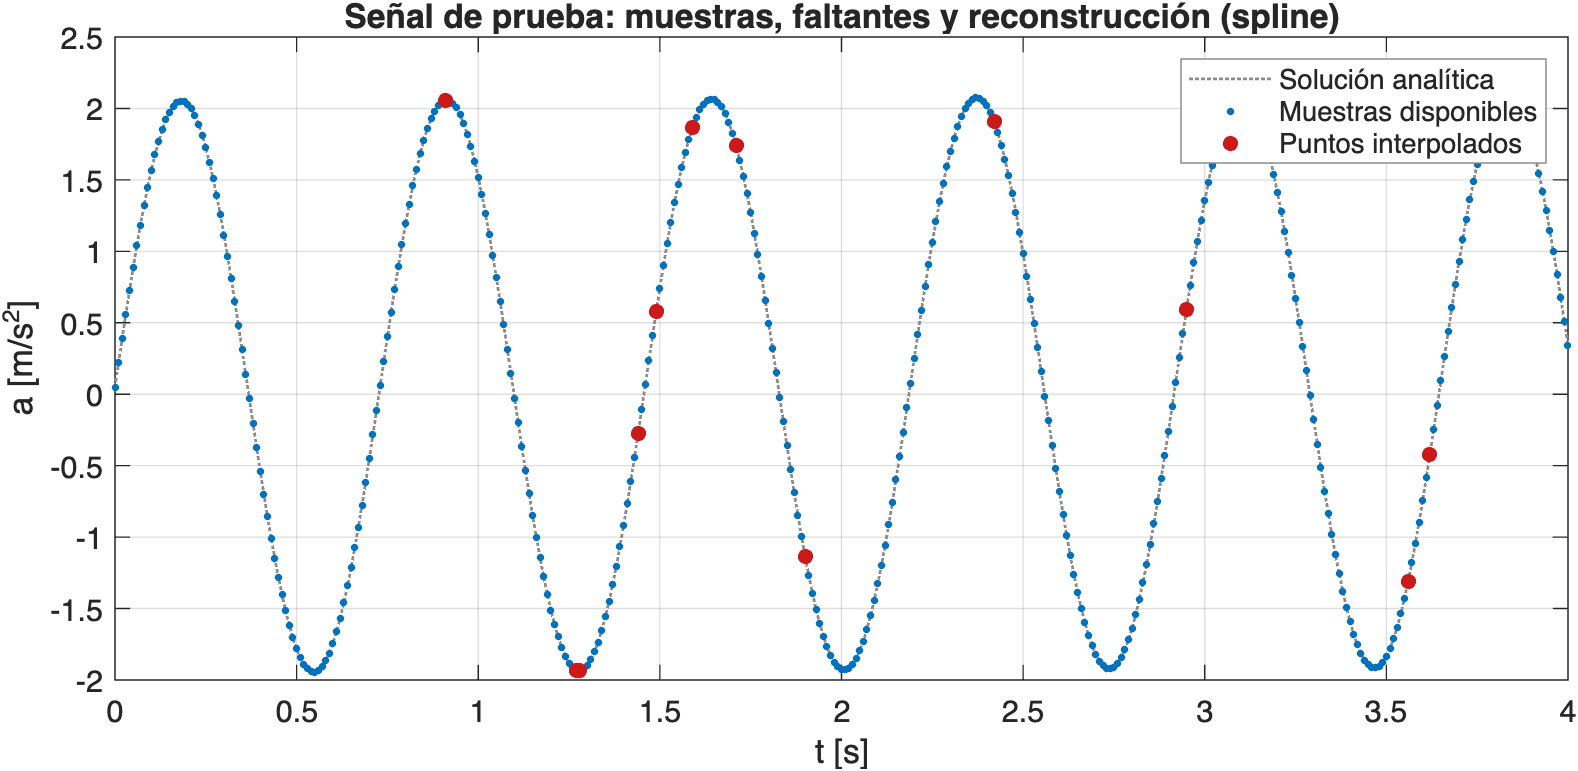
\includegraphics[width=0.9\linewidth]{f01_senal_prueba_faltantes.png}
\figurenote{Puntos azules: muestras disponibles. Puntos rojos: valores reconstruidos con el trazador cúbico natural. Línea punteada: solución analítica. Se muestran los primeros 4~s de 10~s.}
\end{figure}

\begin{table}[htbp]
\caption{Error de cada método contra la solución analítica}
\label{tab:validacion}
\centering\small
\begin{tabular}{@{}llccc@{}}
\toprule
Proceso & Método & Error & Orden observado & Orden teórico \\
\midrule
\multirow{3}{*}{Interpolación (máx.)} & Lineal & $1.48\times10^{-2}$ & -- & -- \\
 & Newton local cúbico & $5.48\times10^{-5}$ & -- & -- \\
 & Trazador natural & $3.01\times10^{-5}$ & -- & -- \\
\midrule
\multirow{4}{*}{Derivada ($h = 0.1$)} & Adelante & $5.00\times10^{-2}$ & 1.00 & 1 \\
 & Atrás & $5.00\times10^{-2}$ & 1.00 & 1 \\
 & Centrada & $3.32\times10^{-3}$ & 2.00 & 2 \\
 & Cinco puntos & $1.97\times10^{-5}$ & 3.99 & 4 \\
\midrule
\multirow{3}{*}{Integral ($n = 12$)} & Trapecio & $1.14\times10^{-2}$ & 2.00 & 2 \\
 & Simpson 1/3 & $5.26\times10^{-5}$ & 4.00 & 4 \\
 & Simpson 3/8 & $1.19\times10^{-4}$ & 4.01 & 4 \\
\midrule
\multirow{3}{*}{EDO, $x(t)$ ($h = 0.01$)} & Euler & $1.34\times10^{-2}$ & 1.11 & 1 \\
 & Heun & $1.42\times10^{-3}$ & 2.00 & 2 \\
 & RK4 & $1.93\times10^{-6}$ & 3.94 & 4 \\
\midrule
\multirow{2}{*}{Mínimos cuadrados} & Grados 1--4 vs.\ \texttt{polyfit} & $\le 3.3\times10^{-14}$ & -- & -- \\
 & Gauss con pivoteo vs.\ \texttt{A\textbackslash b} & $< 10^{-10}$ & -- & -- \\
\bottomrule
\end{tabular}
\figurenote{Resultados de \texttt{prueba\_metodos.m} ejecutado en \matlab{}. El orden observado es la pendiente de $\log E$ contra $\log h$ con cuatro valores de $h$ (tres para la EDO). En la EDO el orden se estimó con solo tres valores de $h$, por lo que el 1.11 de Euler, ligeramente mayor que el teórico, se encuentra dentro de la incertidumbre de esa estimación.}
\end{table}

\begin{figure}[htbp]
\caption{Convergencia de los métodos de derivación, integración y solución de la EDO}
\label{fig:convergencia}
\centering
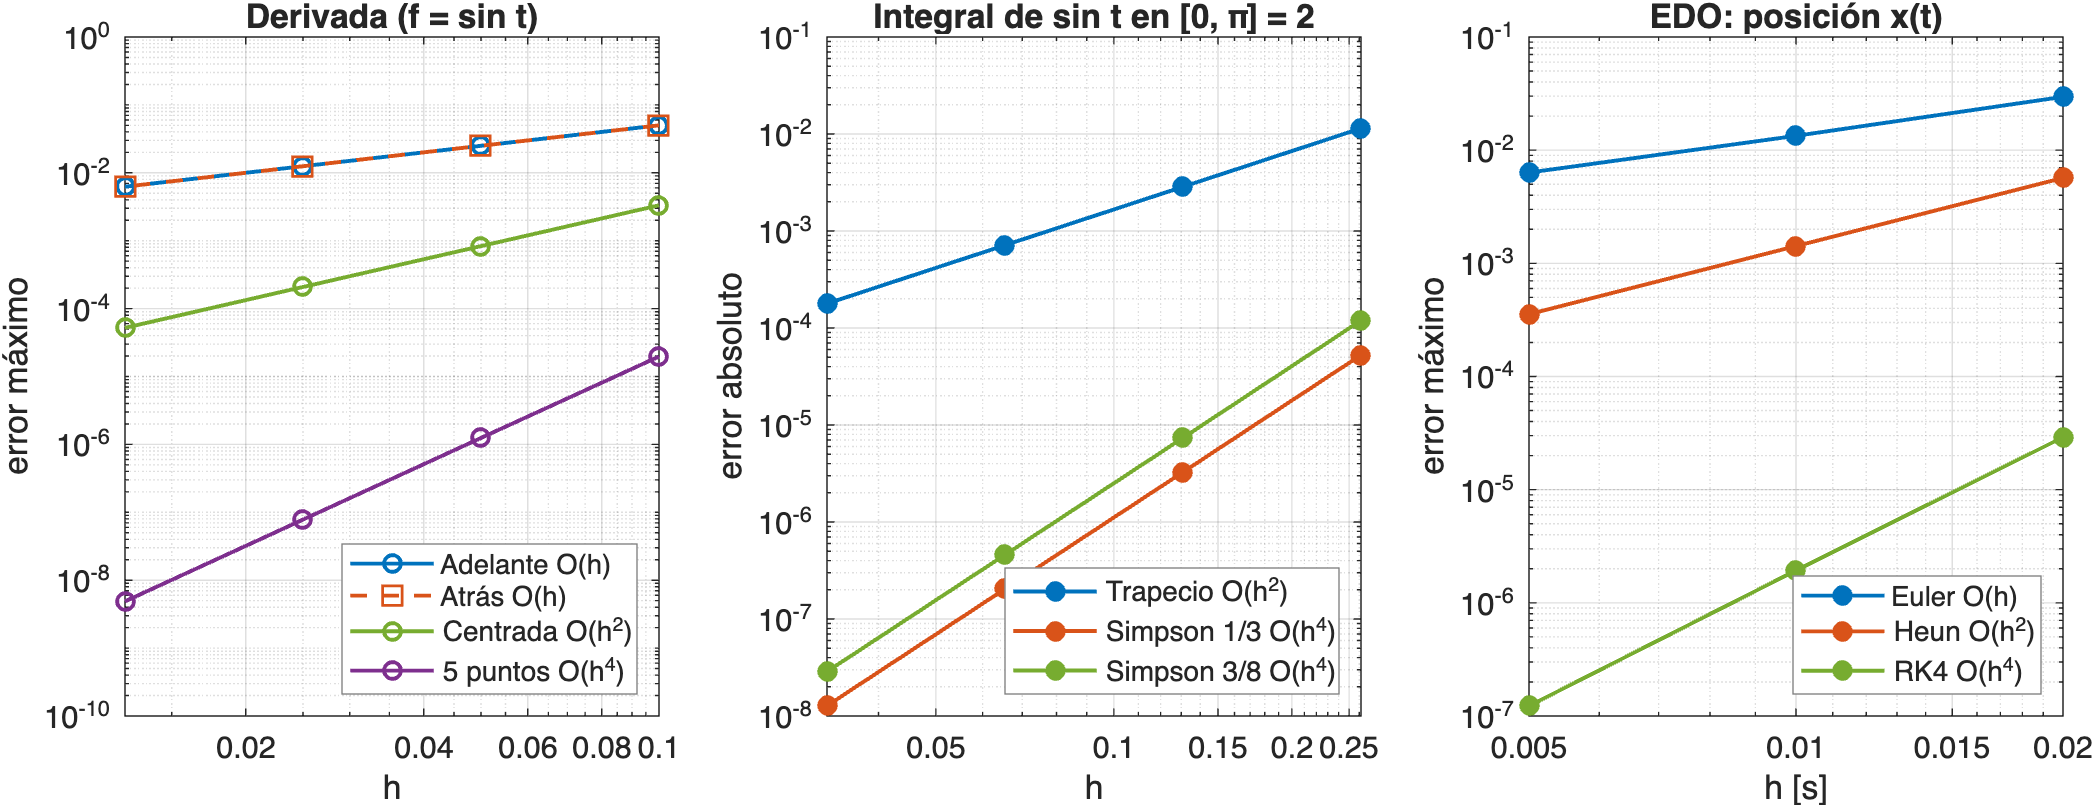
\includegraphics[width=\linewidth]{f02_convergencia.png}
\figurenote{Escalas logarítmicas. La pendiente de cada recta es el orden de convergencia. Las curvas de adelante y atrás coinciden porque ambas fórmulas tienen el mismo error máximo para $\sin t$.}
\end{figure}

\subsection{Duración y datos faltantes en las mediciones reales}

Las tres mediciones duraron entre 63.5 y 78.5~s, con un paso de muestreo de 0.01000~s y una variación (\textit{jitter}) de solo $1.7\times10^{-6}$~s (Tabla~\ref{tab:mediciones}). Ninguna tenía valores NaN ni huecos temporales. El filtro de Hampel detectó dos atípicos en el eje $z$ del cofre, ninguno en la cabina y cinco en el eje $x$ del manejo; cuatro de estos últimos alrededor de $t = 24.24$~s.

\subsection{Vibración del motor}

La Figura~\ref{fig:cofre} muestra la aceleración vertical sobre el cofre. El acercamiento de 0.4~s deja ver una oscilación regular con cerca de cuatro muestras por ciclo. El espectro (Figura~\ref{fig:espectro}) tiene un pico dominante en $f = 25.26$~Hz en los tres ejes; con la ecuación~\eqref{eq:rpm}, eso equivale a unas 758~rpm. En la cabina, media hora después, el pico apareció en 22.86~Hz (686~rpm), junto con su segundo armónico en 45.74~Hz, que es la componente dominante del eje $y$.

\begin{figure}[htbp]
\caption{Aceleración vertical medida sobre el cofre con el motor en ralentí}
\label{fig:cofre}
\centering
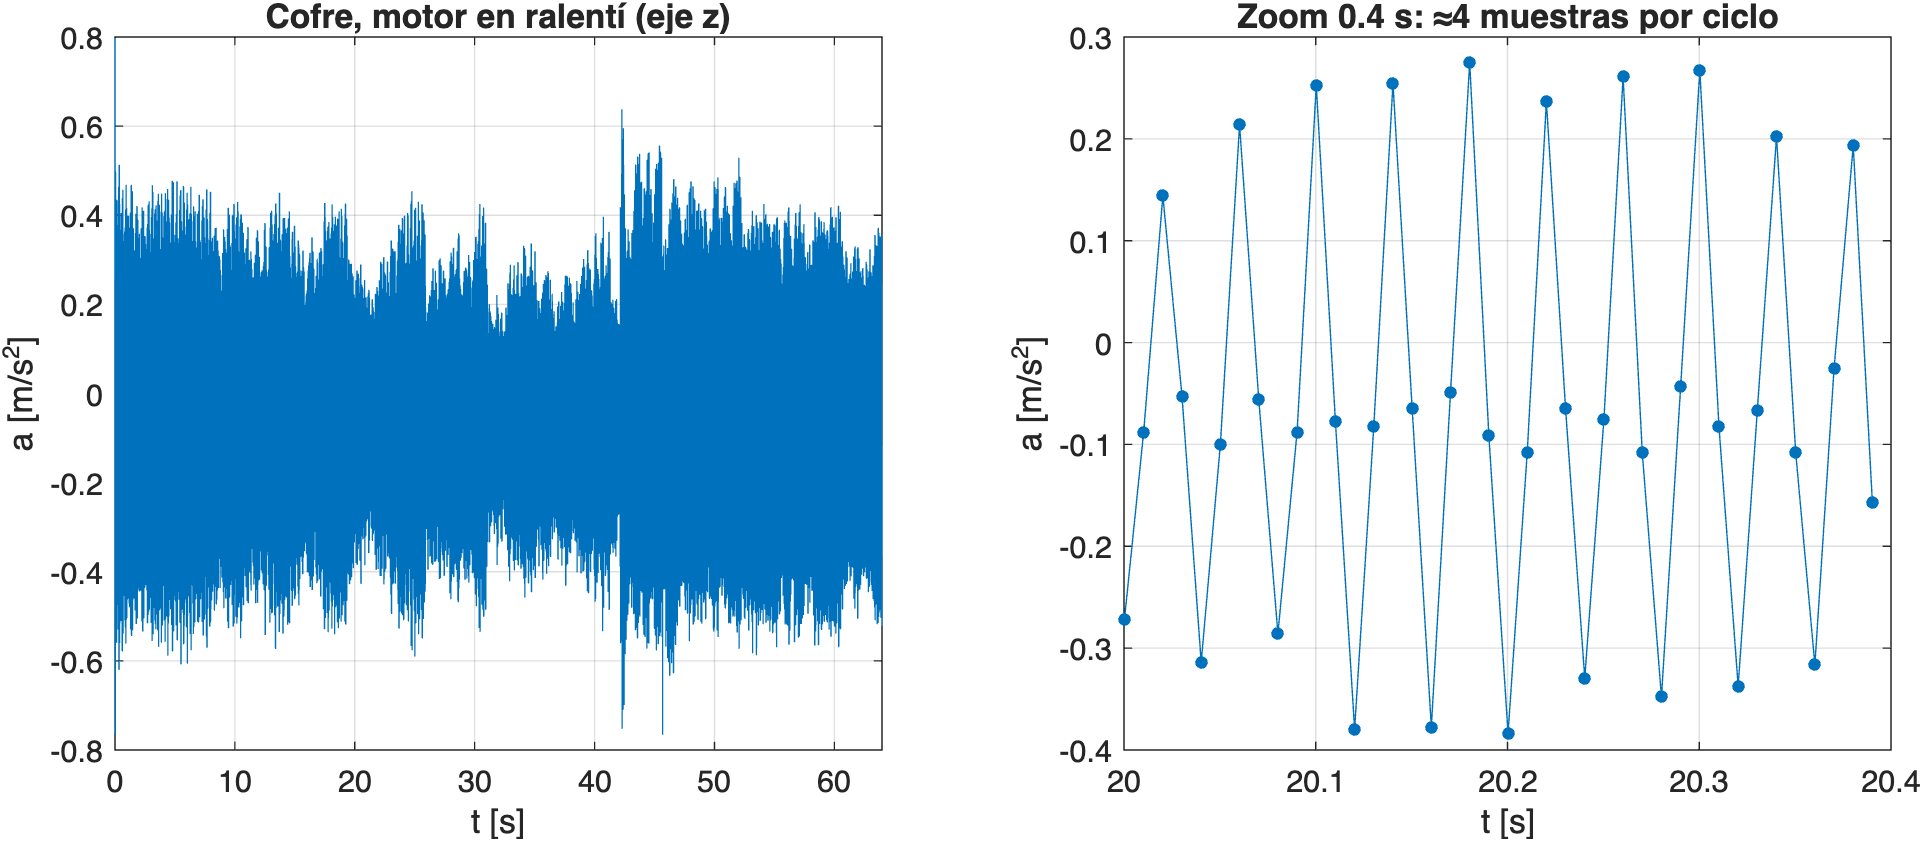
\includegraphics[width=\linewidth]{f03_cofre_senal_y_zoom.png}
\end{figure}

\begin{figure}[htbp]
\caption{Espectro de la vibración vertical en el cofre y en la cabina}
\label{fig:espectro}
\centering
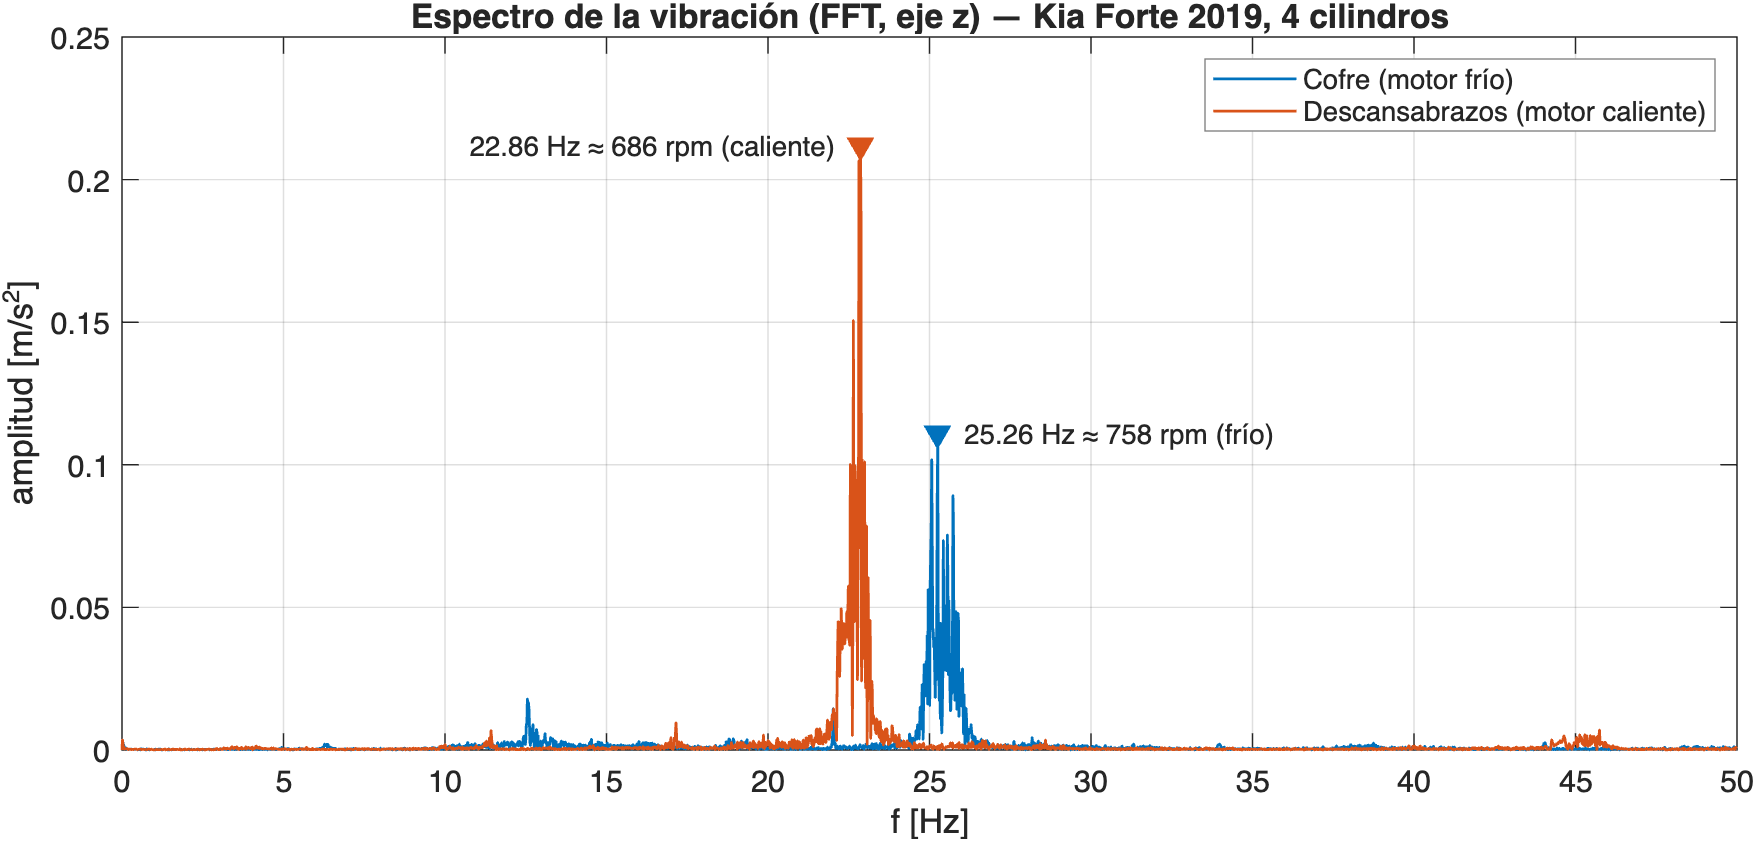
\includegraphics[width=0.95\linewidth]{f04_espectro_cofre_vs_cabina.png}
\figurenote{Espectro de amplitud de un lado calculado con FFT sobre toda la señal (resolución de 0.016~Hz).}
\end{figure}

Al analizar la señal del cofre en ventanas de 8~s, la frecuencia bajó de 25.75 a 25.00~Hz en el primer minuto (Tabla~\ref{tab:rpm}, Figura~\ref{fig:rpm}). Con el motor recién encendido, la unidad de control eleva el ralentí y lo reduce conforme el motor se calienta, que es lo que muestra la secuencia de mediciones. El espectro independiente de phyphox dio 22.65~Hz en la cabina, a 0.2~Hz del valor de esta aplicación. Esa diferencia es menor que la resolución de phyphox (0.39~Hz) y constituye una validación cruzada contra otro programa.

\begin{table}[htbp]
\caption{Frecuencia dominante y velocidad de ralentí estimada}
\label{tab:rpm}
\centering\small
\begin{tabular}{@{}llcc@{}}
\toprule
Hora & Medición & $f$ [Hz] & rpm ($=30f$) \\
\midrule
11:22 & Cofre, ventana 0--8~s (esta aplicación) & 25.75 & 773 \\
11:23 & Cofre, ventana 48--56~s (esta aplicación) & 25.00 & 750 \\
11:22--11:23 & Cofre, señal completa (esta aplicación) & 25.26 & 758 \\
11:26 & Cofre, \textit{Acceleration Spectrum} (phyphox) & 23.05 & 692 \\
11:54 & Cabina, señal completa (esta aplicación) & 22.86 & 686 \\
11:55 & Cabina, \textit{Acceleration Spectrum} (phyphox) & 22.65 & 680 \\
\bottomrule
\end{tabular}
\end{table}

\begin{figure}[htbp]
\caption{Velocidad de ralentí estimada en función del tiempo desde el arranque}
\label{fig:rpm}
\centering
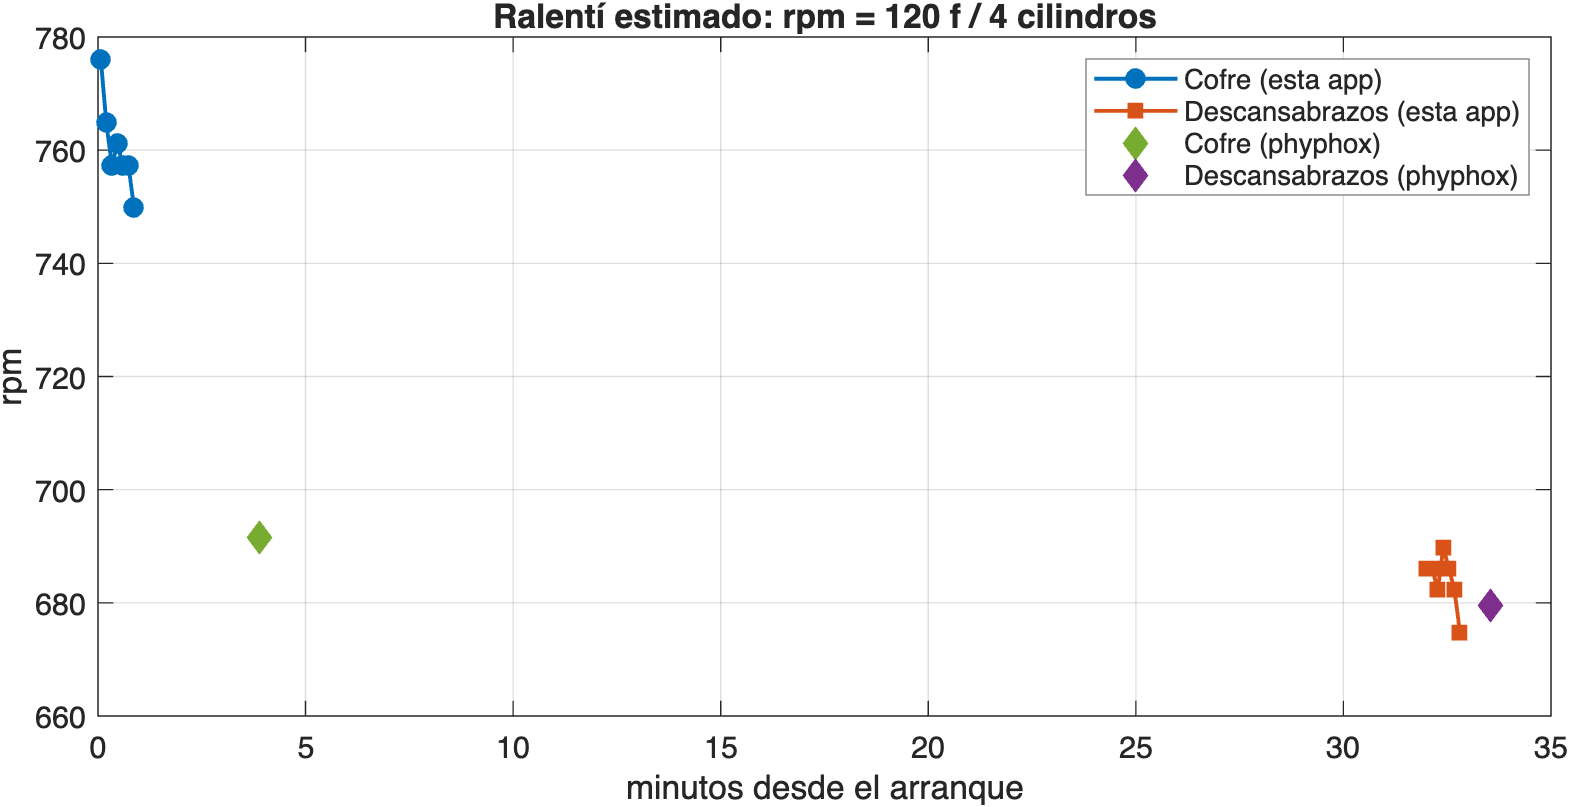
\includegraphics[width=0.85\linewidth]{f05_rpm_vs_tiempo.png}
\end{figure}

La amplitud no se comportó como se esperaba. La hipótesis era que la cabina vibraría menos que el cofre gracias a los soportes del motor, pero el valor RMS del eje $z$ fue de 0.430~m/s$^2$ en la cabina contra 0.289~m/s$^2$ en el cofre. La tapa plástica del descansabrazos es un panel ligero que puede amplificar la vibración, y además las dos mediciones se tomaron con el motor a velocidades distintas, de modo que con estos datos no se puede cuantificar el aislamiento de los soportes.

\subsection{Interpolación sobre datos reales}

La Tabla~\ref{tab:interp} y la Figura~\ref{fig:interp} comparan el error de reconstrucción al eliminar el 5\,\% de las muestras. En las tres mediciones reales el método lineal tuvo el menor error y el trazador cúbico el mayor, justo al revés que con la señal sintética.

\begin{table}[htbp]
\caption{Error RMS de interpolación con 5\,\% de muestras eliminadas [m/s$^2$]}
\label{tab:interp}
\centering\small
\begin{tabular}{@{}lccc@{}}
\toprule
Señal & Lineal & Newton local cúbico & Trazador natural \\
\midrule
Cofre, eje $z$ & \textbf{0.412} & 0.579 & 0.623 \\
Cabina, eje $z$ & \textbf{0.621} & 0.880 & 0.898 \\
Manejo, eje $x$ & \textbf{0.595} & 0.871 & 1.042 \\
Sintética (error máximo) & $1.5\times10^{-2}$ & $5.5\times10^{-5}$ & $\mathbf{3.0\times10^{-5}}$ \\
\bottomrule
\end{tabular}
\figurenote{Datos reales: semilla 1 de \texttt{prueba\_datos\_reales.m} en \matlab{}, entre 320 y 395 muestras evaluadas por señal. La Figura~\ref{fig:interp} usa el promedio de cinco semillas.}
\end{table}

\begin{figure}[htbp]
\caption{Error de interpolación por método y por señal}
\label{fig:interp}
\centering
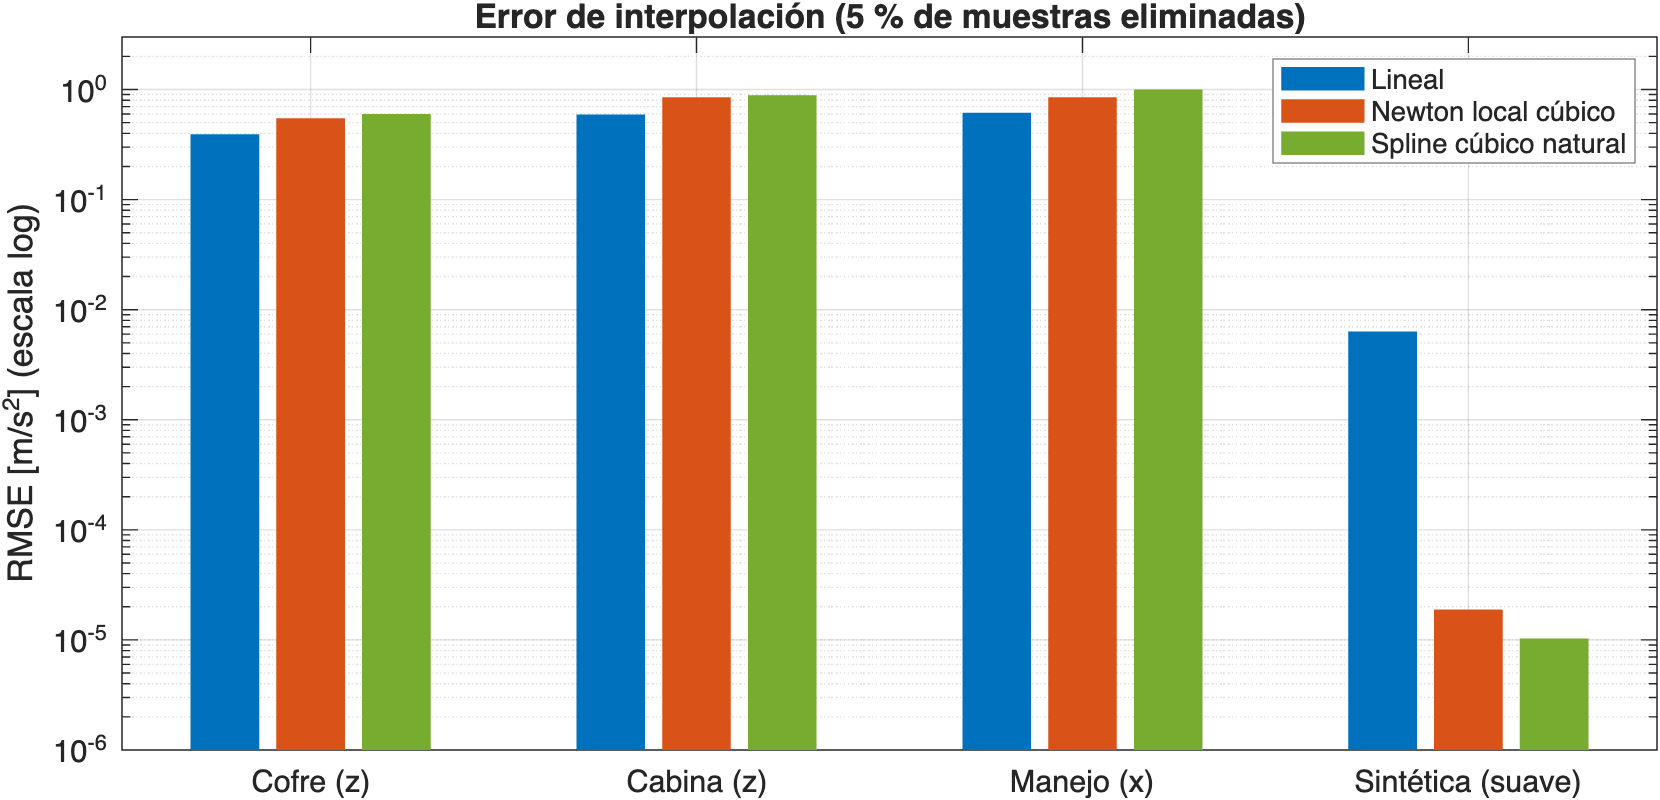
\includegraphics[width=0.9\linewidth]{f07_interpolacion_rmse.png}
\end{figure}

\subsection{Valores atípicos}

En la medición de manejo, en $t = 24.24$~s aparece una sola muestra de $-29.4$~m/s$^2$ (unas 3~$g$), mientras que las vecinas rondan 1~m/s$^2$ (Figura~\ref{fig:atipico}). El filtro de Hampel la detectó y la reconstruyó, y el pico máximo del eje $x$ bajó de 25.3 a 3.5~m/s$^2$. La primera versión del programa usaba un umbral global (mediana y MAD de toda la señal) y marcaba 106 «atípicos» en el eje $z$, que en realidad eran baches del camino. El criterio local de Hampel resolvió ese problema (bitácora, entrada 17).

\begin{figure}[htbp]
\caption{Pico aislado detectado con el filtro de Hampel en la medición de manejo}
\label{fig:atipico}
\centering
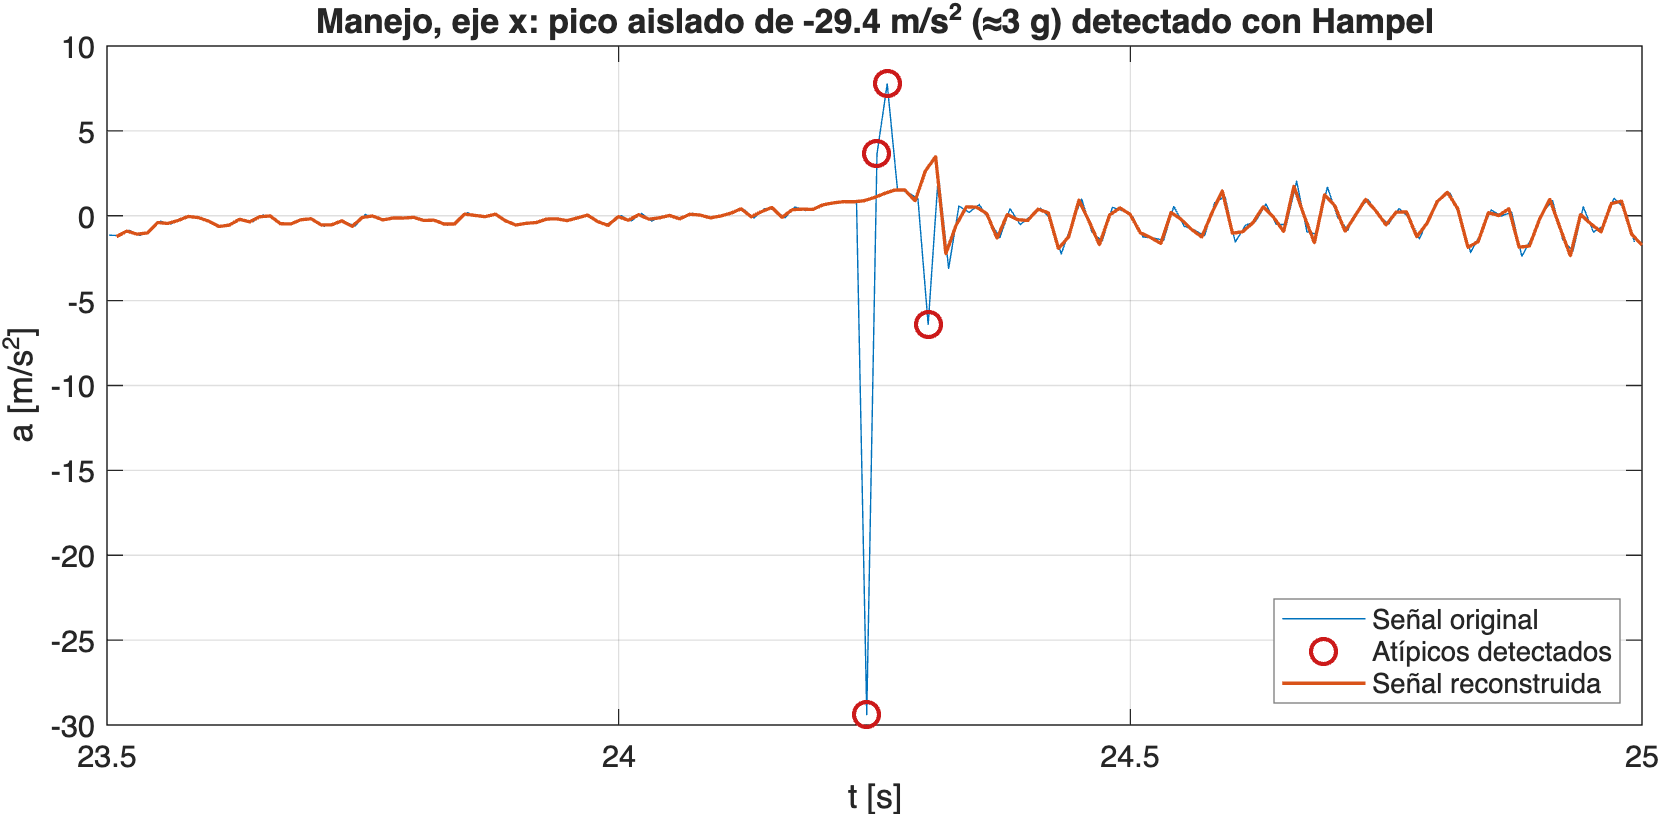
\includegraphics[width=0.9\linewidth]{f08_atipico_hampel.png}
\end{figure}

\subsection{Derivada de la señal}

Con la vibración del motor, $f/f_s = 0.253$ y $\theta = 1.587$~rad. Según la ecuación~\eqref{eq:factor}, la derivada centrada conserva solo el 63.0\,\% de la amplitud real del \textit{jerk}, la de cinco puntos el 84.3\,\% y la de adelante el 89.8\,\%, esta última con un desfase de 45.5$^\circ$ (Figura~\ref{fig:factor}). En la señal del cofre, el \textit{jerk} máximo fue de 109.3~m/s$^3$ con la fórmula centrada, 110.8 con la de cinco puntos y 93.6 con la de adelante.

\begin{figure}[htbp]
\caption{Fracción de la amplitud que conserva cada fórmula de derivación}
\label{fig:factor}
\centering
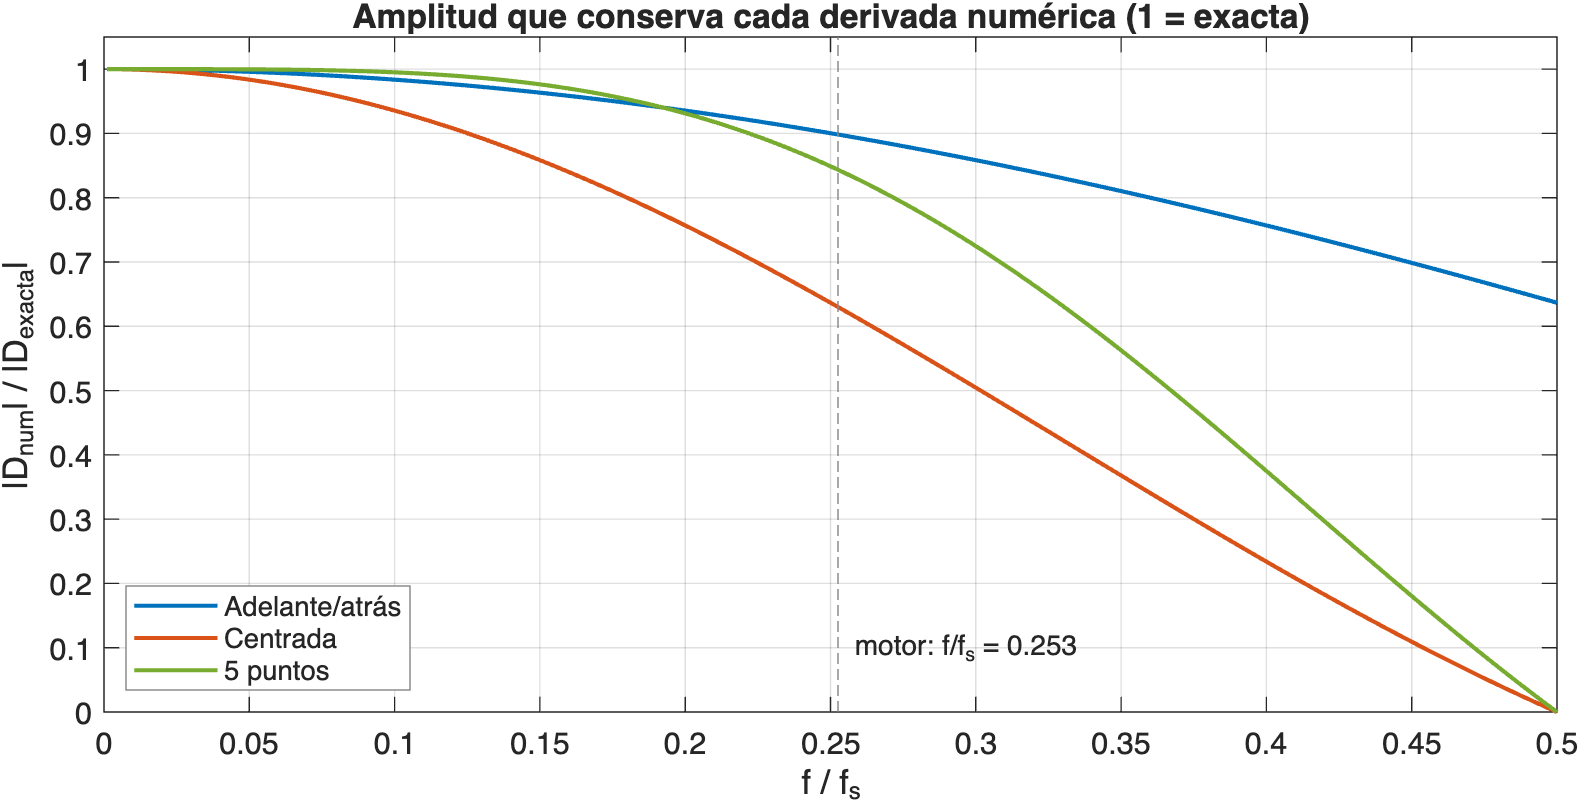
\includegraphics[width=0.85\linewidth]{f09_factor_derivadas.png}
\figurenote{La línea discontinua marca la frecuencia del motor en ralentí (25.26~Hz) con $f_s = 100$~Hz.}
\end{figure}

\subsection{Integral, ecuación diferencial y deriva}

Con el vehículo estacionado la velocidad y el desplazamiento reales son prácticamente nulos, lo que da una referencia exacta para evaluar la integración. Sin corrección, la integral de la aceleración del cofre indica que el vehículo alcanzó 4.09~m/s y se desplazó 127~m (Tabla~\ref{tab:deriva}, Figura~\ref{fig:deriva}). El sesgo medido fue $\hat b = -0.0639$~m/s$^2$; la ecuación~\eqref{eq:deriva} predice $\Delta v = 4.09$~m/s y $\Delta x = 130.8$~m, valores que concuerdan con lo observado, así que el error se debe casi por completo al sesgo. Restar la tendencia de grado 1 redujo el desplazamiento final a 0.31~m, más de 400 veces menos.

\begin{table}[htbp]
\caption{Velocidad y desplazamiento integrados con RK4 según la corrección de deriva}
\label{tab:deriva}
\centering\small
\begin{tabular}{@{}llccc@{}}
\toprule
Medición & Corrección & $v(T)$ [m/s] & $|v|_{\max}$ [m/s] & $x(T)$ [m] \\
\midrule
\multirow{3}{*}{Cofre (estacionado)} & Ninguna & $-4.094$ & 4.094 & $-127.23$ \\
 & Sesgo constante (MC grado 0) & $-0.006$ & 0.088 & 3.54 \\
 & Tendencia MC grado 1 & $-0.006$ & 0.031 & $\mathbf{-0.31}$ \\
\midrule
\multirow{3}{*}{Cabina (estacionado)} & Ninguna & $-5.246$ & 5.246 & $-163.08$ \\
 & Sesgo constante & 0.001 & 0.093 & 3.60 \\
 & Tendencia MC grado 1 & 0.001 & 0.020 & $\mathbf{0.12}$ \\
\midrule
\multirow{3}{*}{Manejo, eje $x$} & Ninguna & 4.446 & 5.335 & 180.25 \\
 & Sesgo constante & 0.002 & 2.758 & 5.77 \\
 & Tendencia MC grado 1 & 0.002 & 2.654 & 0.18 \\
\bottomrule
\end{tabular}
\figurenote{En el manejo se activó el filtro de Hampel. En ese caso la posición no representa el recorrido real del vehículo, porque el eje del teléfono no estaba alineado con la dirección de avance.}
\end{table}

\begin{figure}[htbp]
\caption{Velocidad y posición integradas del vehículo estacionado (cofre, eje $z$)}
\label{fig:deriva}
\centering
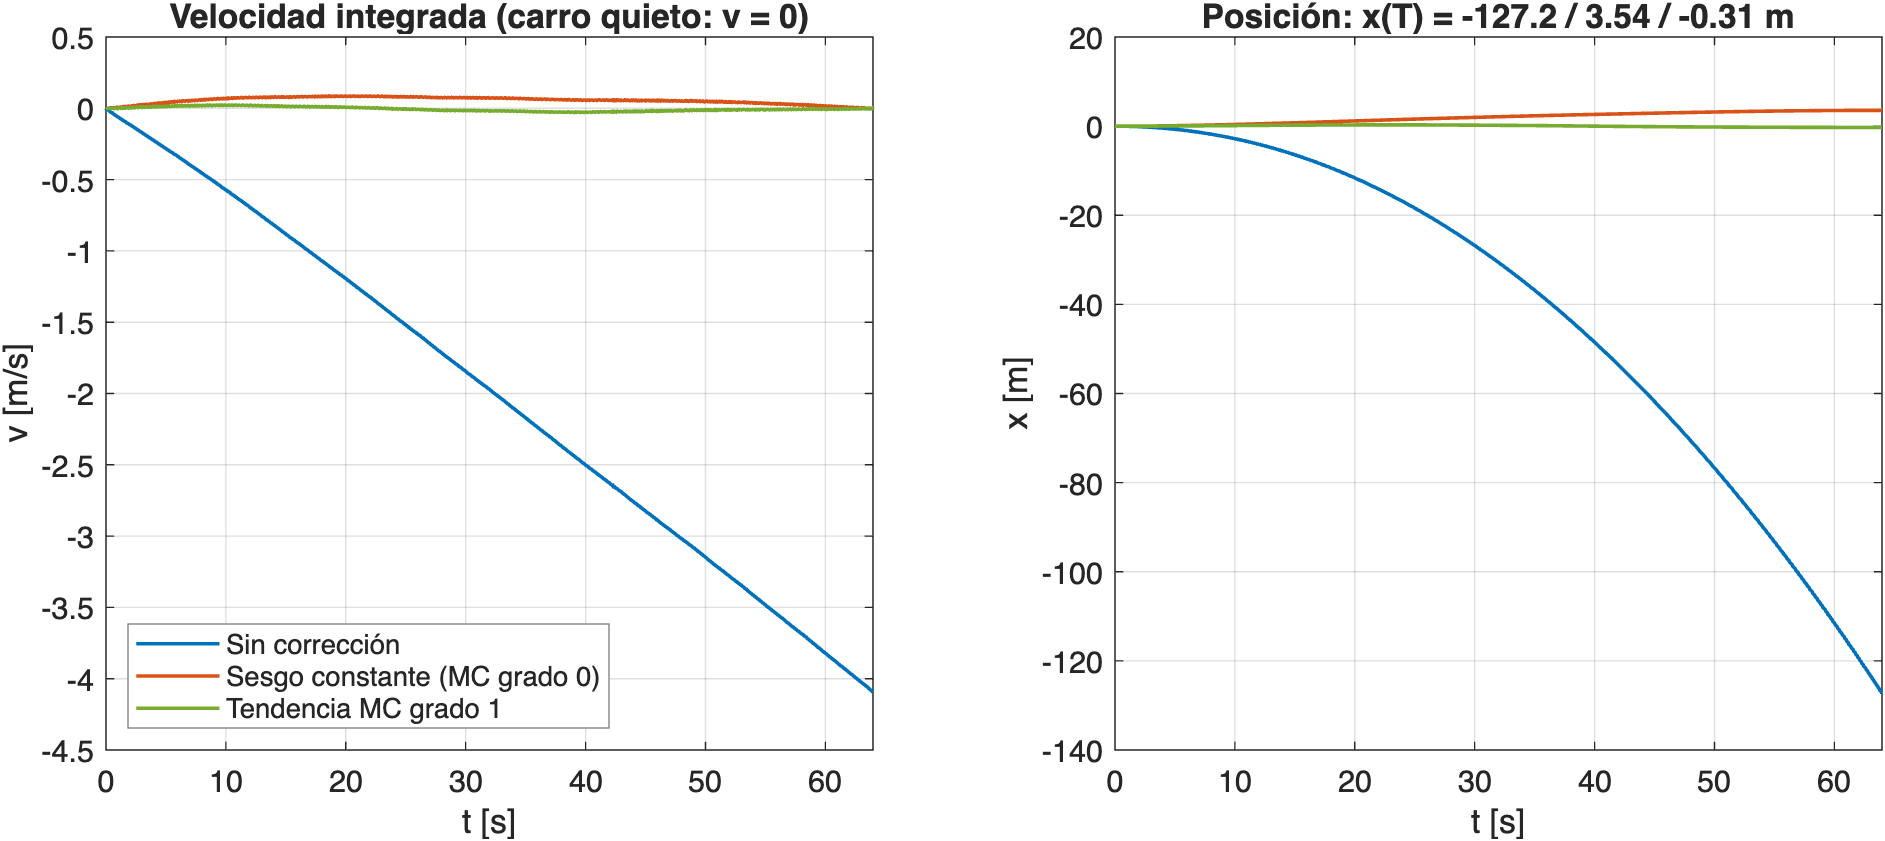
\includegraphics[width=\linewidth]{f06_drift_velocidad_posicion.png}
\end{figure}

Las tres reglas de integración aplicadas a la señal real sin corregir dieron valores casi iguales en el cofre: $-4.288$ (trapecio), $-4.282$ (Simpson 1/3) y $-4.294$~m/s (Simpson 3/8), con diferencias menores al 0.15\,\%. En la ecuación diferencial, Heun y la integral doble con \texttt{cumtrapz} difirieron solo $5\times10^{-5}$~m. Es lo esperado, porque cuando $\mathbf{f}$ no depende del estado Heun se reduce a la regla del trapecio. RK4 y Euler difirieron de esa referencia en 0.03 y 0.30~m, respectivamente.

La Figura~\ref{fig:manejo} presenta la velocidad del eje $x$ del teléfono durante el manejo. Sin corrección la velocidad termina en 16~km/h; con el sesgo constante regresa a cero, aunque toma valores negativos porque el eje del teléfono no coincidía con la dirección de avance del vehículo.

\begin{figure}[htbp]
\caption{Velocidad integrada en el eje $x$ del teléfono durante el manejo}
\label{fig:manejo}
\centering
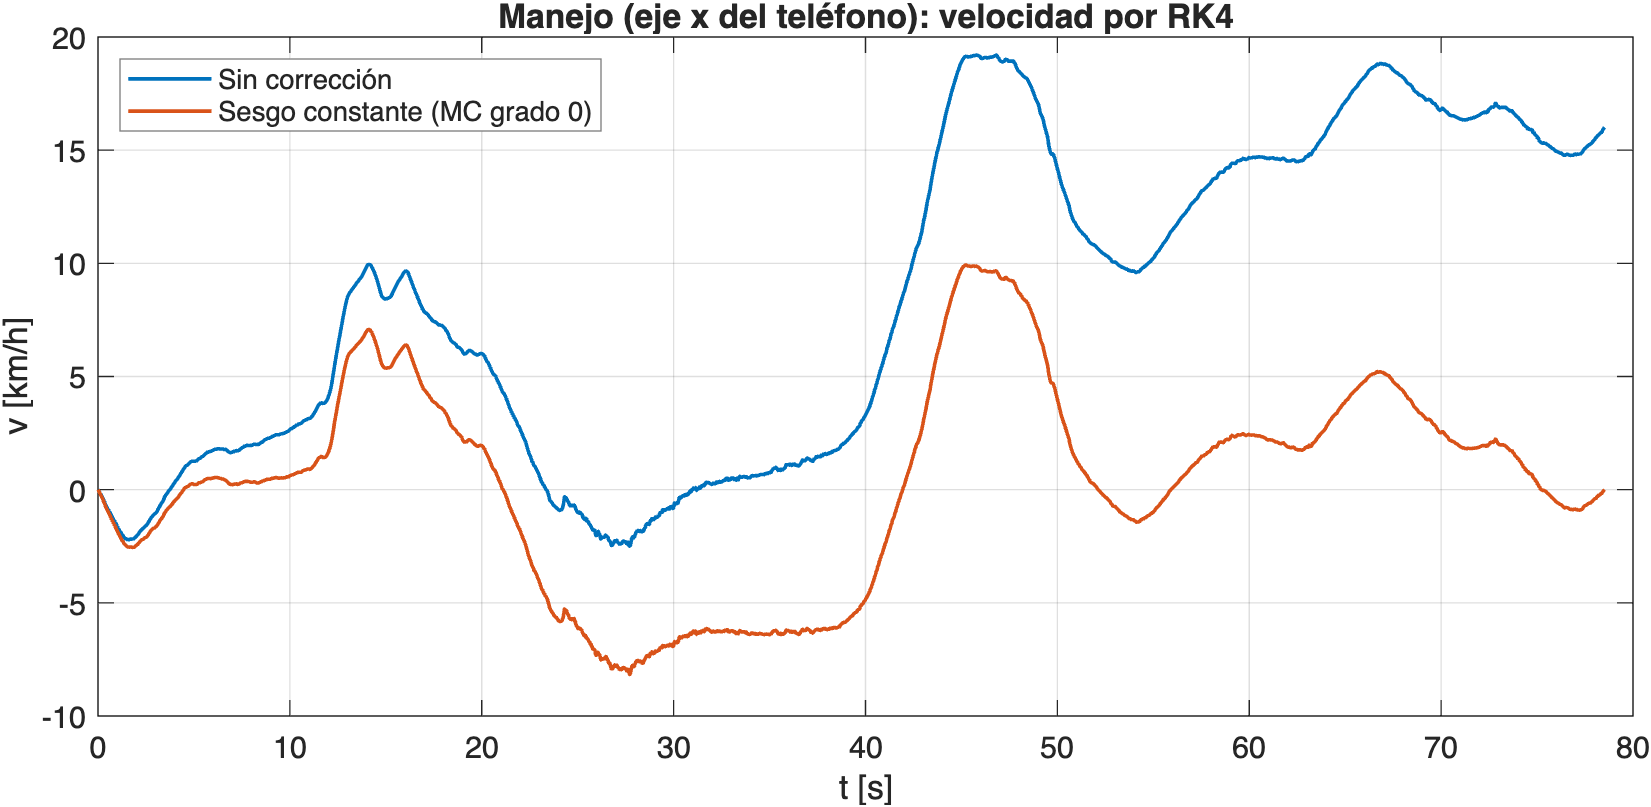
\includegraphics[width=0.9\linewidth]{f10_manejo_velocidad.png}
\end{figure}

\subsection{Línea de tendencia por mínimos cuadrados}

Las tendencias de grado 1 a 3 sobre la señal de manejo tienen coeficientes de determinación muy bajos, de $R^2 = 0.0000$, $0.0023$ y $0.0073$ (Figura~\ref{fig:tendencia}). Esto es lo correcto: la tendencia no pretende explicar la vibración, que oscila alrededor de cero, sino separar el sesgo y la deriva lenta del sensor. Gracias a la variable escalada, el número de condición de la matriz normal fue de 1.0, 7.6, 35.8 y 211.5 para los grados 1 a 4. Sin escalamiento, la matriz de Vandermonde con $t$ entre 0 y 80~s tendría números de condición de muchos órdenes de magnitud más.

\begin{figure}[htbp]
\caption{Líneas de tendencia por mínimos cuadrados sobre la señal de manejo}
\label{fig:tendencia}
\centering
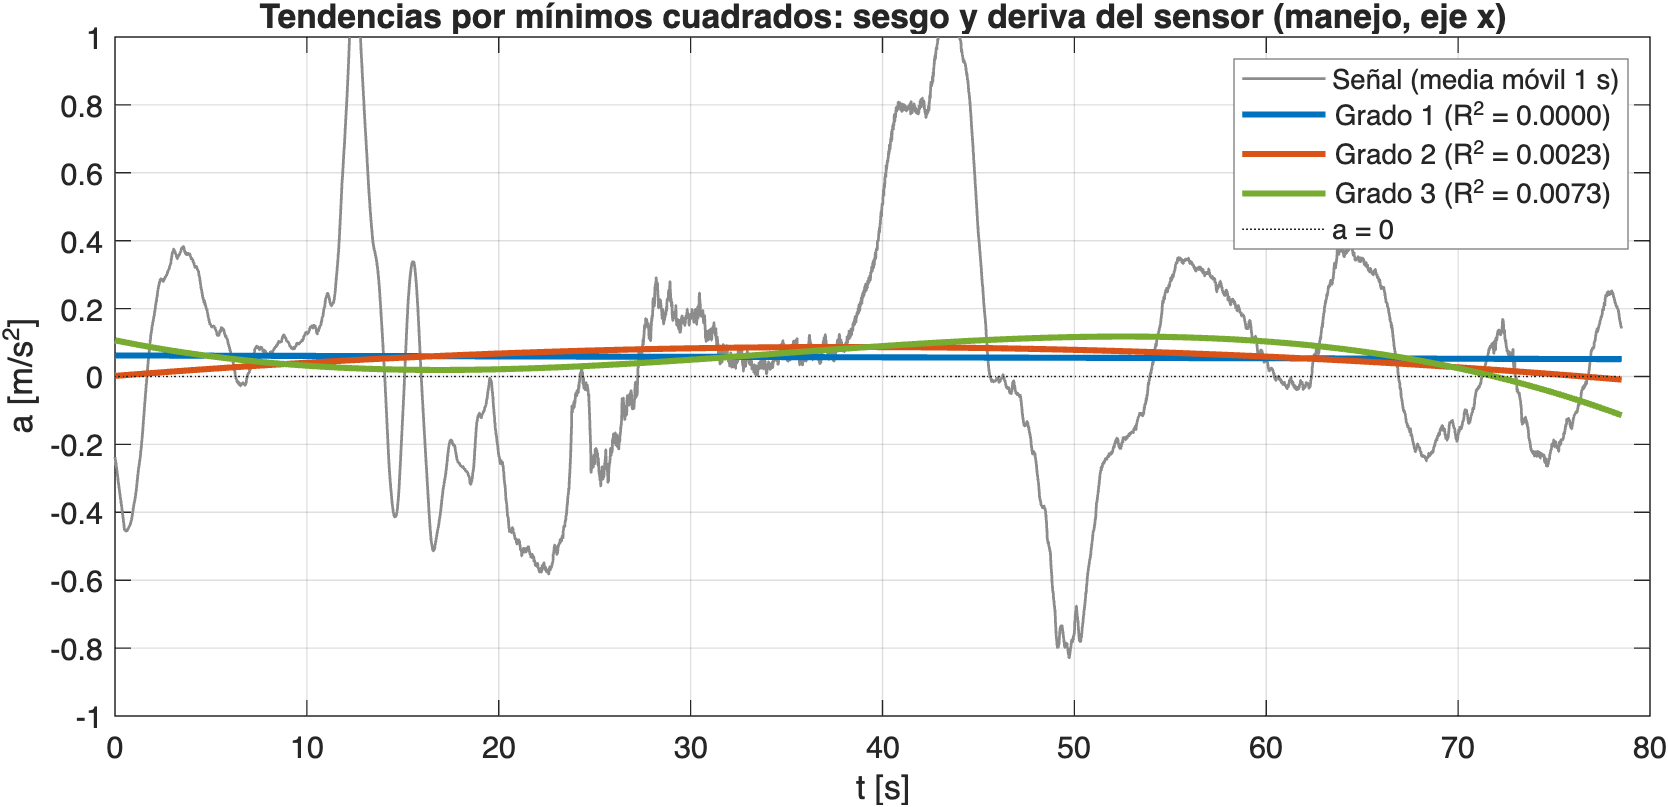
\includegraphics[width=0.9\linewidth]{f11_tendencia_mc.png}
\end{figure}

\subsection{Funcionamiento de la aplicación}

Las Figuras~\ref{fig:app} a~\ref{fig:foto} muestran la aplicación en funcionamiento con los datos reales: el panel de control, la reproducción en tiempo real durante una grabación, la validación de métodos y los archivos exportados.

\begin{figure}[htbp]
\caption{Interfaz del analizador con la medición del cofre}
\label{fig:app}
\centering
\captura{app_general.png}{\linewidth}{captura de la ventana completa con \texttt{motor\_ralenti\_cofre.csv}, eje $z$, tema claro}
\figurenote{Izquierda: panel de control. Arriba: datos originales. Centro: señal procesada. Abajo: resultados.}
\end{figure}

\begin{figure}[htbp]
\caption{Monitor en tiempo real durante una grabación}
\label{fig:tiemporeal}
\centering
\captura{app_tiempo_real.png}{\linewidth}{captura de la pestaña \textit{Tiempo real} con la grabación activa (segmento en rojo e indicador encendido)}
\end{figure}

\begin{figure}[htbp]
\caption{Pestaña de validación de métodos con datos reales}
\label{fig:appvalidacion}
\centering
\captura{app_validacion.png}{\linewidth}{captura de la pestaña \textit{Validación de métodos} después de pulsar \textit{Comparar todos los métodos}}
\end{figure}

\begin{figure}[htbp]
\caption{Exportación de resultados con nombre definido por el usuario}
\label{fig:exportacion}
\centering
\captura{app_exportacion.png}{0.48\linewidth}{diálogo de guardado con el nombre escrito}\hfill
\captura{app_archivos.png}{0.48\linewidth}{carpeta con el .xlsx y los PNG claro/oscuro exportados}
\end{figure}

\begin{figure}[htbp]
\caption{Fotografía de la aplicación en funcionamiento}
\label{fig:foto}
\centering
\captura{foto_app_funcionando.jpg}{0.8\linewidth}{fotografía de la computadora ejecutando la aplicación}
\end{figure}
